%
% 2-rueckprojektion.tex
%
% (c) 2022 Prof Dr Andraes Müller, OST Ostschweizer Fachhochschule
%
\section{Rückprojektion
\label{buch:radon:section:rueckprojektion}}
\kopfrechts{Rückprojektion}
Sei $u\colon \mathbb{R}^n\to\mathbb{C}$ eine Funktion und
$\mathscr{R}u\colon \mathbb{R}\times S^{n-1}\to\mathbb{C}$
die Radon-Transformierte.
Ändert man die Funktion $u$ in einer kleinen Umgebung eines Punkts $y$,
dann ändert die Radon-Transformiert nur für diejenigen Hyperbenen,
die in der Nähe von $y$ vorbeigehen.
Daraus kann man schliessen, dass genau die Werte
$\mathscr{R}(\omega\cdot y,\omega)$ Information über den Wert der
Funktion $u$ im Punkt $y$ enthalten.
Sie enthalten aber auch noch Information über alle anderen Punkte.

\begin{definition}[Rückprojektion]
Die {\em Rückprojektion} $\mathscr{R}^*f$ einer Funktion
\index{Rückprojektion}%
$f\colon \mathbb{R}\times S^{n-1}\to\mathbb{C}$ ist die Funktion
\[
(\mathscr{R}^*f)(y)
=
\int_{S_+^{n-1}} f(\omega\cdot y,\omega)\,d\omega.
\]
$\mathscr{R}^*$ heisst auch die {\em duale Transformation}.
\index{duale Transformation}%
\index{Transformation, dual}%
\end{definition}

Die Rückprojektion ist also der Mittelwert der Werte von $f$ über
alle Richtungen, aber in der Entfernung von $y$ vom Nullpunkt.
Wenn $f$ die Radon-Transformierte $f=\mathscr{R}u$ einer Funktion $u$
ist, dann ist die Rückprojektion $(\mathscr{R}^*\mathscr{R}u)(y)$
der Mittelwert aller Werte von $\mathscr{R}u$, die durch Integration
entlang einer Hyperbene durch $y$ entstanden sind.
In der Rückprojektion sind also alle Werte von $u$ gemittelt, aber
der Wert im Punkt $y$ hat besonders grosses Gewicht.
Die duale Transformation ist somit eine erste Approximation für $u$.
Abbildung~\ref{buch:radon:rueckprojektion:fig:rueckprojektion}
zeigt das Resultat der Rückprojektion im Teilbild unten rechts.
In den weiteren Entwicklungen hoffen wir, daraus eine exakte Rekonstruktion
von $u$ zu konstruieren.

%
% Rückprojektion und Ableitungen
%
\subsection{Rückprojektion und Ableitungen}
%
% rueckprojecktion.tex
%
% (c) 2023 Prof Dr Andreas Müller
%
\begin{figure}
\centering
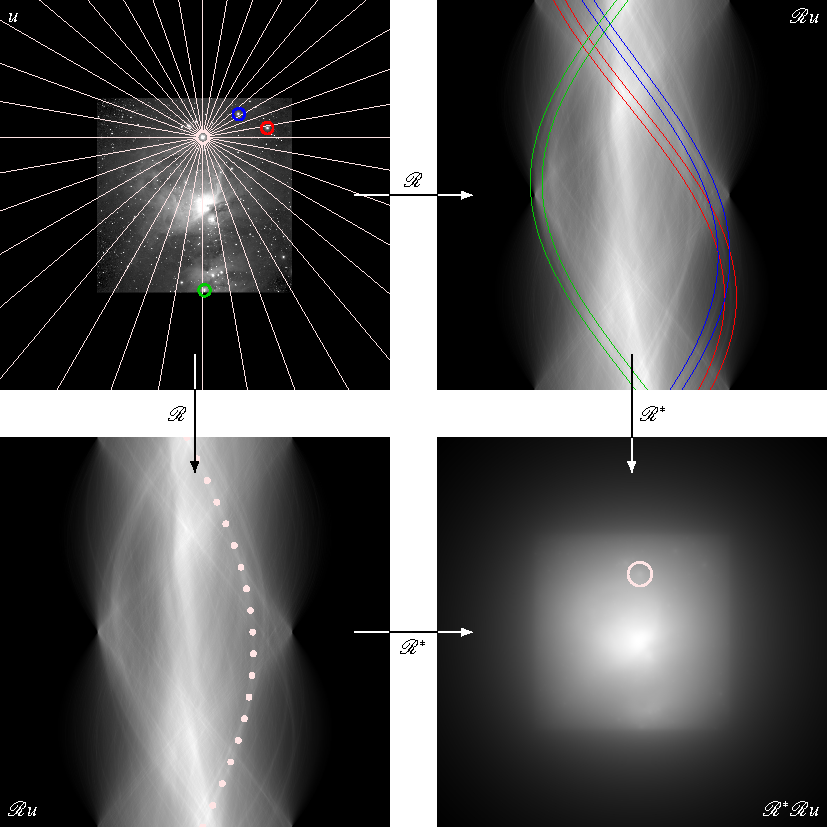
\includegraphics[width=\textwidth]{chapters/050-radon/images/rueckprojektion.pdf}
\caption{Die Rückprojektion $\mathscr{R}^*$ ist eine erste Approximation
der inversen der Radon-Transformation.
In der Radontransformation werden helle Punkte des Bildes zu hellen
sinusähnlichen Kurven (forbig hervorgehobene Kurven in der Radon-Transformation
oben rechts).
Die Punkte einer solchen Kurve stehen für ein Integral über eine
Gerade, die durch den hellen Punkt gehen.
Summiert man diese Punkte (hellrote Punkte in der Radon-Transformation
unten rechts), entsteht ein höherer Wert als entlang einer weniger hellen
Kurve.
Überlagert sind aber auch Anteile von anderen Bildteilen, so entsteht
ein verschwommenes Bild, die Rückprojektion $\mathscr{R}^*u$.
\label{buch:radon:rueckprojektion:fig:rueckprojektion}}
\end{figure}

In diesem Abschnitt ist $v\colon \mathbb{R}\times S^{n-1}\to\mathbb{C}$
eine differenzierbare Funktion mit kompaktem Träger, so dass alle
im Folgenden betrachteten Integrale und Ableitungen existierten.
Aus der Definition
\begin{align*}
\mathscr{R}^*v(x)
&=
\int_{S_+^{n-1}} v(\omega\cdot x,\omega)\,d\omega
\intertext{kann man jetzt auch die Ableitung nach $x_i$ berechnen und
bekommt}
\frac{\partial}{\partial x_i}\mathscr{R}^*v(x)
&=
\int_{S_+^{n-1}}
\frac{\partial}{\partial x_i} v(\omega\cdot x,\omega)\,d\omega
\\
&=
\int_{S_+^{n-1}}
\omega_i
\frac{\partial v}{\partial s}(\omega\cdot x,\omega)
\,d\omega.
\end{align*}
Für den Laplace-Operator findet man dann
\begin{align}
\Delta\mathscr{R}^*v
&=
\int_{S_+^{n-1}}
\underbrace{
\biggl(\sum_{i=1}^n \omega_i^2\biggr)
}_{\displaystyle=1}
\frac{\partial^2 v}{\partial s^2}(\omega\cdot x,\omega)
\,d\omega
\notag
\\
&=
\mathscr{R}^*
\frac{\partial^2}{\partial s^2} v
\qquad\Rightarrow\qquad
\Delta\mathscr{R}^* = \mathscr{R}^*\frac{\partial^2}{\partial s^2}.
\label{buch:radon:rueckprojektion:eqn:laplacedual}
\end{align}
In Satz
\ref{buch:radon:ableitungen:satz:laplace}
wurde gezeigt, wie der Laplace-Operator mit der Radon-Transformation
vertauscht.
Damit kann jetzt aus der
Formel~\ref{buch:radon:rueckprojektion:eqn:laplacedual}
die Identität
\begin{equation}
\Delta\mathscr{R}^*\mathscr{R}u
=
\mathscr{R}^*\frac{\partial^2}{\partial s^2}\mathscr{R}u
=
\mathscr{R}^*\mathscr{R}\Delta u
\end{equation}
gewinnen.

%
% Rückprojektion und die Umkehrformel
%
\subsection{Rückprojektion und die Umkehrformel}
%
% orion2.tex
%
% (c) 2023 Prof Dr Adnreas Müller
%
\begin{figure}
\centering
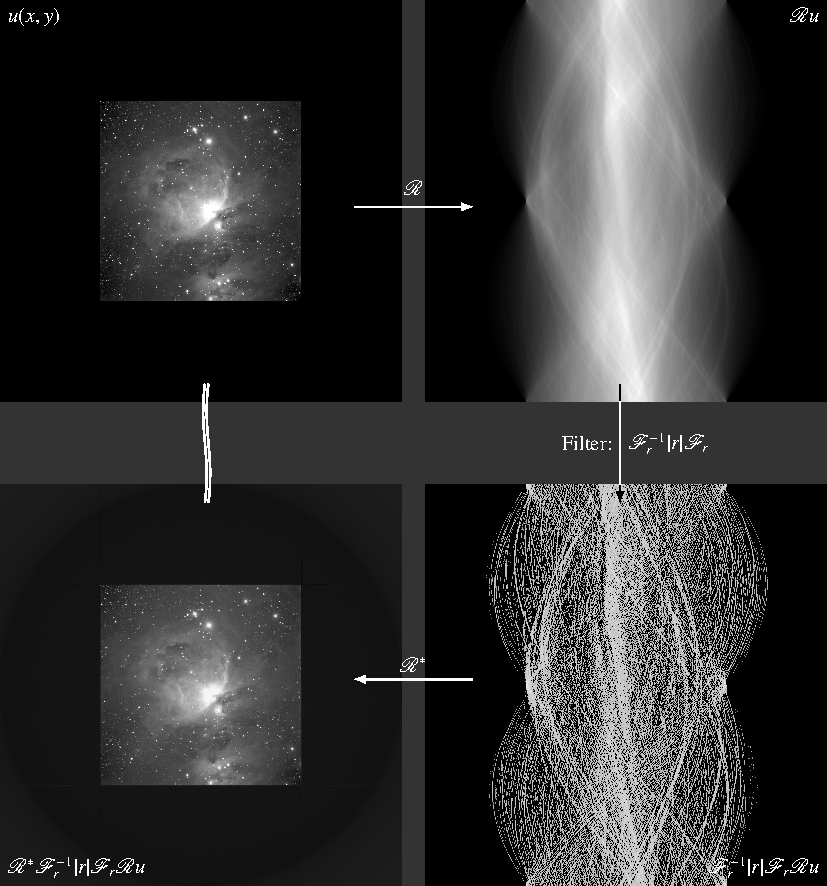
\includegraphics[width=\textwidth]{chapters/050-radon/images/orion2.pdf}
\caption{Rekonstruktion eines Bildes $u$ aus der Radon-Transformierten
$\mathscr{R}u$.
Die Rückprojektion $\mathscr{R}^*\mathbb{R}u$ ist stark verschwommen.
Durch die Anwendung des Filters vor der Rückprojektion kann ein
scharfes und kontrastreiches Bild gewonnen werden.
Die Filterung funktioniert besser, wenn das Bild von einem genügend 
grossen scharzen Gebiet umgeben ist.
\label{buch:radon:rueckprojektion:fig:rueckprojektion}}
\end{figure}

In Abschnitt~\ref{buch:radon:definition:subsection:radon}
haben wir gefunden, dass die Fourier-Transformierte der Funktion $u$
in die Radon-Transformation und eine eindimensionale Fourier-Transformation
zerlegt werden kann.
Dies wird durch die Formel
\[
\mathscr{F}u(k)
=
\frac{1}{(2\pi)^{n/2}}
\int_{\mathbb{R}} 
e^{-i|k|s}
\mathscr{R}u(s,k^0)\,ds
\]
ausgedrückt.
Die Fourier-Umkehrformel ermöglicht, die Funktion aus $\mathscr{F}u$ 
wieder zu berechnen, sie ist
\begin{align*}
u(x)
&=
\frac{1}{(2\pi)^{n/2}}
\int_{\mathbb{R}^n} e^{ik\cdot x}
\mathscr{F}u(k)\,dk.
\intertext{Das Integral über $\mathbb{R}$ kann wieder in den
``Radon-Koordinaten''
$(r,\omega)$ berechnet werden mit $r=|k|$ und $\omega = k^0$.
So entsteht
}
&=
\frac{1}{(2\pi)^{n/2}}
\int_0^\infty
\int_{S^{n-1}} e^{i(r\omega)\cdot x}
\mathscr{F}u(r\omega)
\,d\omega
r^{n-1}
\,dr.
\intertext{Der Faktor $r^{n-1}$ kommt von der Koordinatentransformation.
Das Integral über die Kugeloberfläche $S^{n-1}$ kann in zwei Integrale
über die Halbkugeln
$S_+^{n-1}=\{x\in S^{n-1}\mid x_1\ge 0\}$
und
$S_-^{n-1}=\{-\omega\mid \omega\in S_+^{n-1}\}$
zerlegt werden, die durch die Spiegelung
$S^{n-1}\to S^{n-1}:\omega\mapsto-\omega$ ineinander übergeführt werden.
So erhält man}
&=
\frac{1}{(2\pi)^{n/2}} \int_0^\infty \int_{S_+^{n-1}}
e^{i(r\omega)\cdot x} \mathscr{F}u(r\omega)\,d\omega r^{n-1}\,dr
\\
&\quad+
\frac{1}{(2\pi)^{n/2}} \int_0^\infty \int_{S_+^{n-1}}
e^{i(-r\omega)\cdot x} \mathscr{F}u(-r\omega)\,d(-\omega) r^{n-1}\,dr.
\intertext{Wir möchten das zweite $r$-Integral in ein Integral
über $(-\infty,0)$ verwandeln.
Dazu müssen wir $-r$ an allen Stellen haben.
Wir können gleichzeitig noch das Minuszeichen in $d(-\omega)$ entfernen,
denn die Spiegelung $\omega\mapsto -\omega$ hat die Determinante
$(-1)^{n-1}$. 
Damit wird
}
u(x)
&=
\frac{1}{(2\pi)^{n/2}} \int_0^\infty \int_{S_+^{n-1}}
e^{i(r\omega)\cdot x} \mathscr{F}u(r\omega)\,d\omega r^{n-1}\,dr
\\
&\quad+
\frac{1}{(2\pi)^{n/2}} \int_0^\infty \int_{S_+^{n-1}}
e^{i(-r\omega)\cdot x} \mathscr{F}u(-r\omega)\,(-1)^{n-1}d\omega
(-r)^{n-1}(-1)^{n-1}\,d(-r)
\\
&=
\frac{1}{(2\pi)^{n/2}} \int_0^\infty \int_{S_+^{n-1}}
e^{i(r\omega)\cdot x} \mathscr{F}u(r\omega)\,d\omega r^{n-1}\,dr
\\
&\quad+
(-1)^{n-1}
\frac{1}{(2\pi)^{n/2}} \int_{-\infty}^0 \int_{S_+^{n-1}}
e^{ir\omega\cdot x} \mathscr{F}u(r\omega)
d\omega
|r|^{n-1}\,dr.
\intertext{Jetzt kann man die beiden Integrale in einziges
$r$-Integral
}
u(x)
&=
\frac{1}{(2\pi)^{n/2}}
\int_{\mathbb{R}} \int_{S_+^{n-1}}
e^{ir\omega\cdot x}
\mathscr{F}u(r\omega)
\,d\omega
|r|^{n-1}\,dr
\intertext{über ganz $\mathbb{R}$ zusammenfassen.
Durch Vertauschung der Integrationsreihenfolge
entsteht als inneres Integral die Fourier-Inversionsformel
für eine eindimensionale Fourier-Transformierte:}
u(x)
&=
\frac{1}{(2\pi)^{n/2}}
\int_{S_+^{n-1}}
\int_{\mathbb{R}}
e^{ir\omega\cdot x}
\mathscr{F}u(r\omega)
|r|^{n-1}\,dr
\,
d\omega.
\end{align*}
Das äussere Integral ist die Rückprojektion $\mathscr{R}^*$.
Wir wissen bereits, dass die Fourier-Transformation $\mathscr{F}$
zerlegt werden kann in die Radon-Transformation und die
eindimensionale Fourier-Transformation, die wir früher mit
$\mathscr{F}_r$ bezeichnet haben.
Damit ergibt sich der folgende Satz:

\begin{satz}[Gefilterte Rückprojektion]
Für eine integrierbare Funktion $u\colon\mathbb{R}^n\to\mathbb{C}$ mit kompaktem Träger gilt
\[
u
=
\frac{1}{(2\pi)^{n-1}}
\mathscr{R}^*
\mathscr{F}_r^{-1}
|r|^{n-1}
\mathscr{F}_r
\mathscr{R}u,
\]
wobei der Term $|r|^{n-1}$ der Multiplikationsoperator mit der
Funktion $r\mapsto |r|^{n-1}$ ist.
\end{satz}

Dieser Satz zeigt eine neue Möglichkeit, die Radon-Transformation
zu invertieren.
Dazu muss die $s$-Abhängigkeit der Radon-Transformierten
$\mathscr{R}u(r,\omega)$ 
zunächst mit $\mathscr{F}_r$ in den Frequenzbereich transformiert werden.
Im Frequenzbereich wird mit $|r|^{n-1}$ multipliziert, dadurch
werden die hohen Frequenzen verstärkt.
Schliesslich wird mit $\mathscr{F}_r^{-1}$ in den $s$-Bereich
zurücktransformiert.
Die nachfolgende duale Transformation mit $\mathscr{R}^*$ entsteht
das ursprüngliche Bild.
Die mittleren drei Schritte $\mathscr{F}_r^{-1}|r|^{n-1}\mathscr{F}_r$
entsprechen einer frequenzabhängigen Filterung.
\index{Filterung}%
\index{frequenzabhängige Filterung}%
Der Satz besagt also, dass die Radon-Transformierte zunächst
gefiltert werden muss, um anschliessend mit der Rückprojektion
$\mathscr{R}^*$ die ursprüngliche Funktion zurückzugeben.
Die Zusammensetzung heisst aus diesem Grund die {\em gefilterte
Rückprojektion}.
\index{Rückprojektion!gefiltert}%
\index{gefilterte Rückprojektion}%
Der Prozess wird in
Abbildung~\ref{buch:radon:rueckprojektion:fig:rueckprojektion}
illustriert.

Der Satz macht auch verständlich, warum die Rekunstruktion nicht
unbedingt stabil ist. 
Der Faktor $|r|^{n-1}$ verstärkt Rauschen umso mehr, je höher
die Frequenz ist.
Da weisses Rauschen über das ganze Spektrum gleiche Leistungsdichte
hat (zur Thematik Rauschen und harmonische Analysis siehe auch 
Kapitel~\ref{chapter:brown}),
wird das Resultat vom Rauschen dominiert.
Rauschen ist aber in praktischen Anwendungen unvermeidlich, es
entsteht durch Messfehler aber auch auch durch die unausweichliche
Diskretisation.

Die gefilterte Rückprojektion zeigt aber auch einen Ausweg und 
damit eine praktisch realisierbare Möglichkeit, die Radon-Transformation
zu invertieren.
Dazu wird der Filter $r\mapsto |r|^{n-1}$ für grosse $r$ abgeschnitten,
die Funktion wird also durch eine Funktion ersetzt, die sehr
hohe Frequenzen nicht weiter verstärkt.
Damit verliert man zwar Bildschärfe, bekommt aber das Rauschen unter
Kontrolle.

In Kapitel~\ref{chapter:ct} werden weitere Beispiele zur gefilterten
Rückprojektion und insbesondere Abbildungen gezeigt, die die Wirkung
der Filterung ebenfalls sichtbar machen.

%
% Gefilterte Rückprojektion
%
\subsection{Gefilterte Rückprojektion und Hilbert-Transformation}
Das Stabilitätsproblem bei der Invertierung der Radon-Transformation
kann noch etwas deutlicher gemacht werden, in dem man die gefilterte
Rücktransformation durch die Hilbert-Transformation ausdrückt.
Dieses wird mit einem normalerweise divergenten Integral definiert,
das als der sogenannte Hauptwert interpretiert werden muss.

\begin{definition}[Hauptwert]
Ist $f\colon[a,b]\setminus\{c\}\to\mathbb{R}$ eine stetige Funktion,
dann heisst
\[
\operatorname{PV}
\int_a^b f(x)\,dx
=
\lim_{\varepsilon\to 0+}
\biggl(
\int_a^{b-\varepsilon} f(x)\,dx
+
\int_{b+\varepsilon}^c f(x)\,dx
\biggr)
\]
der {\em Hauptwert} oder {\em principal value} des Integrals.
\index{Hauptwert}%
\index{principal value}%
\end{definition}

Der Hauptwert gibt gewissen uneigentlichen Integralen einen Sinn, 
die mit der konventionellen Definition keinen vernünftigen Wert haben.

\begin{beispiel}
Die Funktion $f\colon x\mapsto 1/x$ ist an der Stelle $x=0$ nicht definiert und
das Integral über das Interval $[-1,1]$ divergiert, wie die folgende Rechnung
zeigt.
Das Integral muss an der Stelle $x=0$ aufgeteilt werden:
\begin{equation}
\int_{-1}^1 f(x)\,dx
=
\lim_{\varepsilon\to 0-}
\int_{-1}^{\varepsilon} \frac{dx}{x}
+
\lim_{\epsilon\to 0+}
\int_{\epsilon}^{1} \frac{dx}{x}.
\label{buch:radon:rueckprojektion:bsp:1x:eqn1}
\end{equation}
Das erste Integral kann mit der Substitution $t=-s$ und $dt=-ds$ vereinfacht
werden zu
\begin{align*}
\int_{-1}^{\varepsilon} \frac{dx}{x}
&=
\int_{1}^{-\varepsilon} \frac{ds}{s}
=
-
\int_{-\varepsilon}^1 \frac{ds}{s}
=
-
\biggl[
\log s
\biggr]_{-\varepsilon}^1
=
-
(
\log 1 - \log(-\varepsilon)
)
=
\log(-\varepsilon).
\end{align*}
Eingesetzt in 
\eqref{buch:radon:rueckprojektion:bsp:1x:eqn1}
erhält man
\[
\int_{-1}^1 f(x)\,dx
=
\lim_{\varepsilon\to 0-}
\log(-\varepsilon)
+
\lim_{\epsilon\to 0+}
(-\log(\epsilon))
=
\underbrace{
\lim_{\varepsilon\to 0+}
\log\varepsilon
}_{\displaystyle\to \infty}
-
\underbrace{
\lim_{\epsilon\to 0+}
\log(\epsilon)
}_{\displaystyle\to \infty}
=
\infty - \infty.
\]
Da nach der konventionellen Definition eines uneigentlichen
Integrals die beiden Grenzwerte unabhängig voneinander genommen werden,
kann dem Integral kein sinnvoller Wert zugewiesen werden.
Dies ändert sich jedoch mit dem Hauptwert, wo die beiden Grenzen
$\varepsilon=\epsilon$ gekoppelt werden.
Dann ergibt sich
\[
\operatorname{PV}
\int_{-1}^1 \frac{dx}{x}
=
\lim_{\varepsilon\to 0+}
\biggl(
\int_{-1}^{-\varepsilon}\frac{dx}{x}
+
\int_{\varepsilon}^{1} \frac{dx}{x}
\biggr)
=
\lim_{\varepsilon\to 0+}
\biggl(
\log\varepsilon - \log\varepsilon
\biggr)
=
0.
\]
Der Hauptwert des Integrals ist also wohldefiniert.
\end{beispiel}

\begin{definition}[Hilbert-Transformation]
Ist $f\colon \mathbb{R}\to\mathbb{C}$ eine stetige und integrierbare
Funktion, dann ist die {\em Hilbert-Trans\-for\-mier\-te} definiert durch
\[
(\mathscr{H}f)(t)
=
\frac{1}{\pi} \operatorname{PV} \int_{-\infty}^\infty \frac{f(t)}{t-x}\,dx,
\]
wobei der {\em Hauptwert} des Integral gleichbedeutend mit
\[
(\mathscr{H}f)(t)
=
\lim_{\varepsilon\to 0+}
\biggl(
\int_{-\infty}^{t-\varepsilon}+\int_{t+\varepsilon}^\infty
\frac{f(x)}{t-x}\,dx
\biggr)
\]
ist.
\end{definition}

Die Definition der Hilbert-Transformation sieht aus wie eine 
Faltung mit der Funktion $x\mapsto 1/x$, da diese aber nicht
integrierbar ist, ist die konventionelle Definition der Faltung
nicht anwendbar.

\begin{satz}[Hilbert-Transformation und Signum]
Die Hilbert-Transformierte $\mathscr{H}f$ einer stetigen Funktion $f$
hat die Fourier-Transformierte
\[
\mathscr{F}\mathscr{H} f
=
-i\sign(k) \mathscr{F}f,
\]
wobei $\operatorname{sign}(r)$ die Multiplikation mit der Vorzeichenfunktion
\[
\sign(k)
=
\begin{cases}
\phantom{+}1&\qquad x > 0\\
\phantom{+}0&\qquad x = 0\\
         - 1&\qquad x < 0
\end{cases}
\]
ist.
\end{satz}

Die Hilbert-Transformation ist im Frequenzbereich die Multiplikation
mit $-i\sign(k)$, während die Ableitung im Frequenzbereich zur Multiplikation
mit $-ik$ wird.
Der Filter der gefilterten Rückprojektion benötigt im Frequenzbereich 
den Faktor $|k|^{n-1}$, 
Diesen kann man wegen $|k|=\sign(k)\cdot k$ aus dem Vorzeichen und der
dem Wert zusammensetzen, d.~h.~für den einfachsten Fall $n=2$ muss man
die Filterung mit
\[
|r|
=
\sign(r)
\cdot r 
=
(-i\sign(r))
\cdot
(-ir)
\]
durchführen.
Die gefilterte Rückprojektionsformel ist
\begin{align*}
u
&=
\frac{1}{2\pi}
\mathscr{R}^*
\mathscr{F}_r^{-1}
|r|
\mathscr{F}_r
\mathscr{R}u
\\
&=
\frac{1}{2\pi}
\mathscr{R}^*
\mathscr{F}_r^{-1}
(-i\sign(r))
\cdot
(-ir)
\mathscr{F}_r
\mathscr{R}u
\\
&=
\frac{1}{2\pi}
\mathscr{R}^*
\mathscr{F}_r^{-1}
(-i\sign(r))
\mathscr{F}_r
\mathscr{F}_r^{-1}
(-ir)
\mathscr{F}_r
\mathscr{R}u
\\
&=
\frac{1}{2\pi}
\mathscr{R}^*
\mathscr{H}
\frac{\partial}{\partial s}
\mathscr{R}u.
\end{align*}
Auch diese Form der gefilterten Rücktransformation illustriert, dass
die Bestimmung der Funktion aus der Radon-Transformation nicht sonderlich
stabil sein kann.
Ist die Radon-Transformierte $\mathscr{R}u$ mit weissem Rauschen verrauscht,
wie das in der Praxis wegen Mess- und Quantisierungsfehlern immer der Fall
ist, dann verstärkt der Operator $\partial/\partial s$ dieses Rauschen
zusätzlich in einem Mass, dass die Rücktransformation möglicherweise schon
die Hilbert-Transformation, spätestens aber die Fourier-Rücktransformation
nicht mehr definiert ist.

